\subsection{Experiment 1}
\label{ssec:exp1}
\addcontentsline{toc}{section}{Experiment 1}

\begin{figure}
\label{fig:exp1-graphs}
\subfloat[Gap size 1]{
    \label{fig:exp1-graphs:1}
    \begin{minipage}[b]{0.5\linewidth}
    \centering
    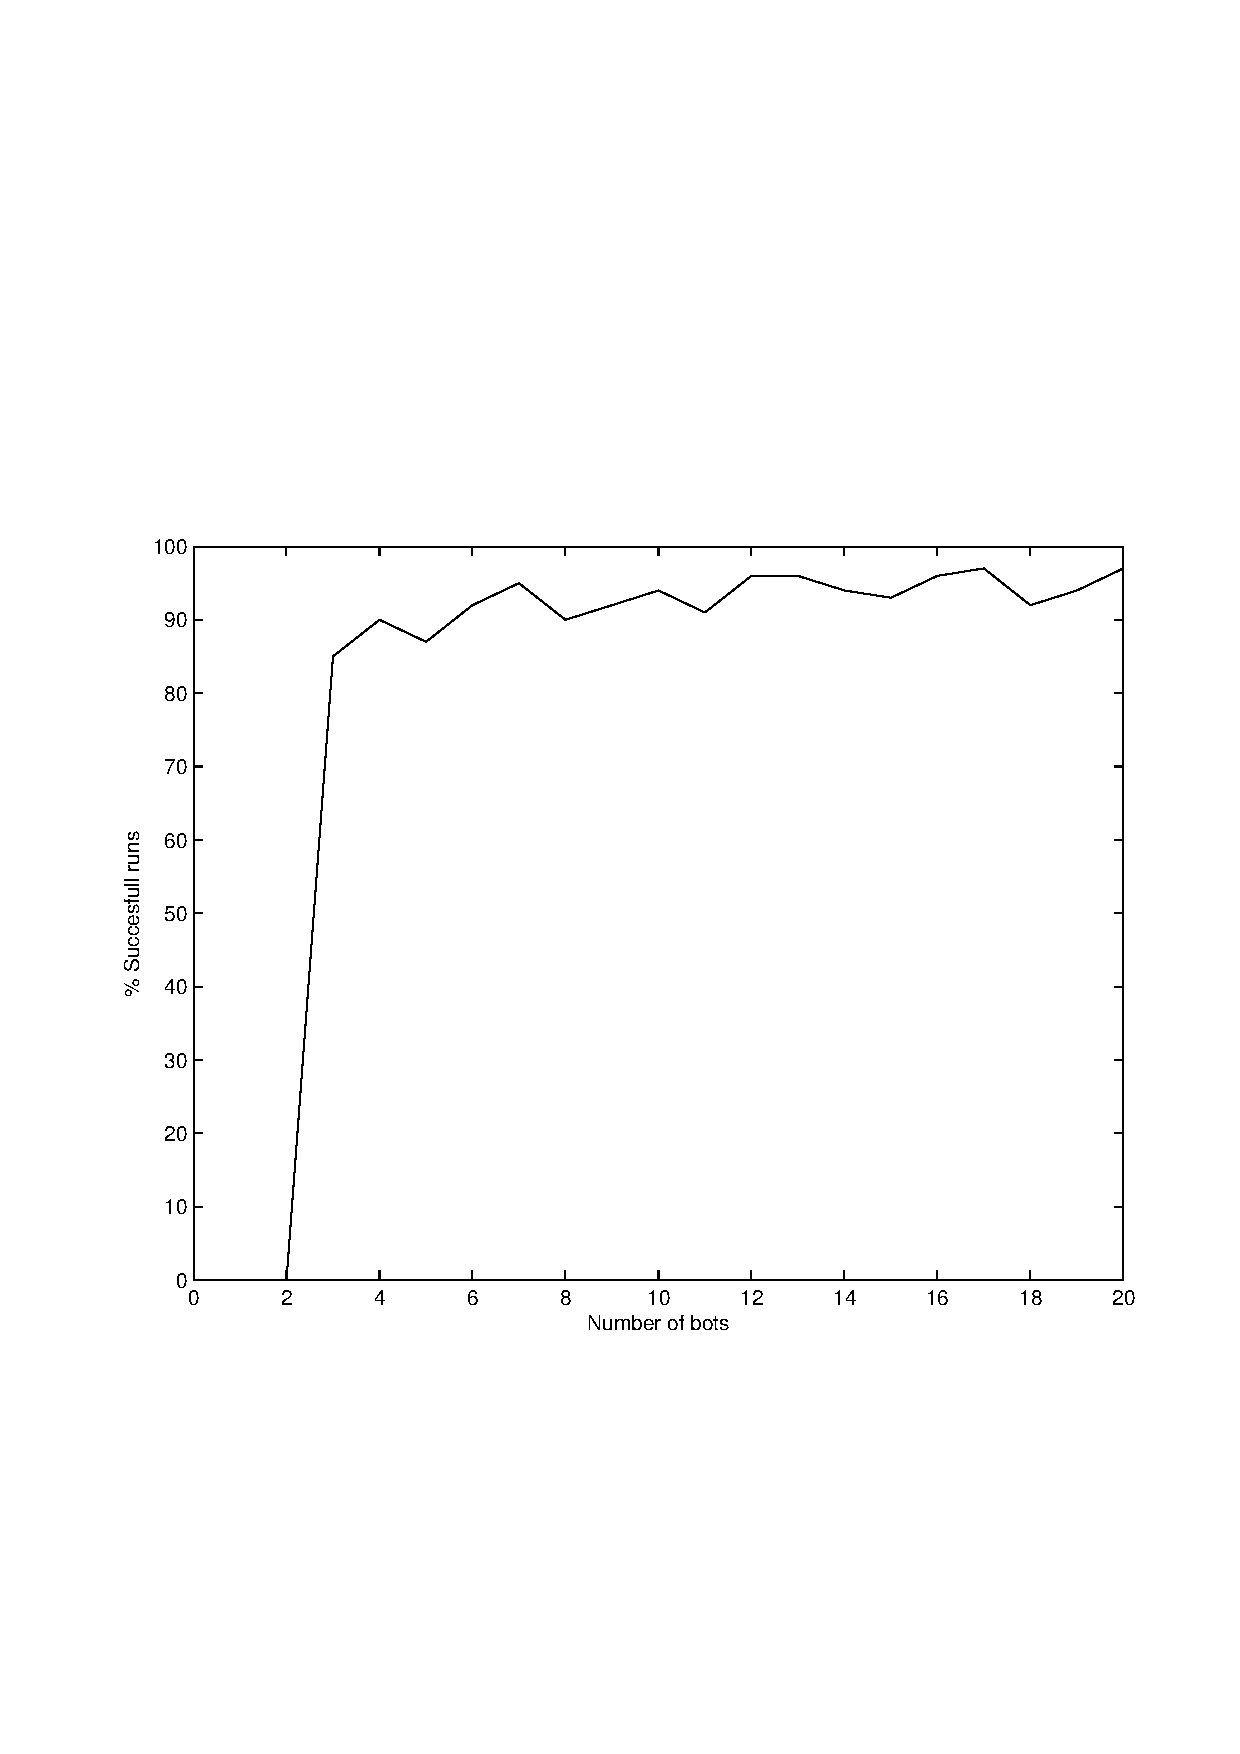
\includegraphics[width=\linewidth]{results/experiment1/plot1}
    \end{minipage}
}%
\hfill
\subfloat[Gap size 2]{
    \label{fig:exp1-graphs:10}
    \begin{minipage}[b]{0.5\linewidth}
    \centering
    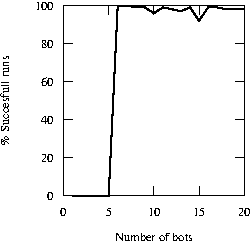
\includegraphics[width=\linewidth]{results/experiment1/plot10}
    \end{minipage}
}
\end{figure}
\begin{table}
 \caption{The variables involved in experiment 1.}
 \begin{center}
  \begin{tabular}{| p{5cm} | c | c |}
   \hline
   \centering \textbf{Variable} & \textbf{Type} & \textbf{Interval} \\ \hline
   gap size & independent & \\ \hline
   box weight & independent & \\ \hline
   number of bots & independent & \\ \hline
   minimum no. of bots & dependent &  \\ \hline
   runs per parameter set & other & \\ \hline
  \end{tabular}
 \end{center}
 \label{tbl:exp1}
\end{table}
